\documentclass[11pt,oneside]{article}

\usepackage[a4paper,margin=26mm,headheight=15pt]{geometry}
\usepackage{fontspec}
\setmainfont{DejaVu Serif}
\setsansfont{DejaVu Sans}
\setmonofont[Scale=0.82]{DejaVu Sans Mono}

\usepackage{microtype}
\usepackage{mathtools,amsthm}
\usepackage{unicode-math}
\setmathfont{DejaVu Math TeX Gyre}
\usepackage{booktabs,longtable,array,tabularx}
\usepackage{enumitem}
\usepackage{xcolor}
\usepackage{tikz}
\usetikzlibrary{arrows.meta,positioning,fit,backgrounds}
\usepackage[most]{tcolorbox}
\usepackage{fvextra}
\usepackage{fancyhdr}
\usepackage{titlesec}
\usepackage{hyperref}
\usepackage{xurl}
\usepackage{bookmark}
\usepackage{cleveref}

\definecolor{Navy}{HTML}{18324B}
\definecolor{Teal}{HTML}{0C6B68}
\definecolor{BlueGray}{HTML}{EAF0F4}
\definecolor{WarmGray}{HTML}{F5F3EF}
\definecolor{Red}{HTML}{9B2C2C}
\definecolor{Green}{HTML}{216E39}
\definecolor{CodeBg}{HTML}{F7F8FA}

\hypersetup{
  colorlinks=true,
  linkcolor=Navy,
  citecolor=Teal,
  urlcolor=Teal,
  pdftitle={Diagonal Ramified Kind-Reflection},
  pdfauthor={Research proposal for the BusyLean project},
  pdfsubject={A proposed computable Lean large number},
  pdfkeywords={Lean, large numbers, reflection, System F omega, W-types}
}

\pagestyle{fancy}
\fancyhf{}
\lhead{Diagonal Ramified Kind-Reflection}
\rhead{BusyLean Contender 11 proposal}
\cfoot{\thepage}
\renewcommand{\headrulewidth}{0.35pt}

\titleformat{\section}{\Large\bfseries\color{Navy}}{\thesection}{0.7em}{}
\titleformat{\subsection}{\large\bfseries\color{Navy}}{\thesubsection}{0.65em}{}
\titleformat{\subsubsection}{\normalsize\bfseries\color{Teal}}{\thesubsubsection}{0.6em}{}

\setlist[itemize]{leftmargin=1.45em,itemsep=2pt,topsep=4pt}
\setlist[enumerate]{leftmargin=1.6em,itemsep=3pt,topsep=4pt}
\setlength{\parindent}{0pt}
\setlength{\parskip}{6pt}
\setlength{\emergencystretch}{2em}

\newtheorem{theorem}{Theorem}[section]
\newtheorem{lemma}[theorem]{Lemma}
\newtheorem{corollary}[theorem]{Corollary}
\newtheorem{proposition}[theorem]{Proposition}
\theoremstyle{definition}
\newtheorem{definition}[theorem]{Definition}
\newtheorem{remark}[theorem]{Remark}

\newtcolorbox{summarybox}[1][]{
  enhanced,breakable,colback=BlueGray,colframe=Navy,
  boxrule=0.7pt,arc=1.5mm,left=3mm,right=3mm,top=2mm,bottom=2mm,
  title=#1,fonttitle=\bfseries
}
\newtcolorbox{statusbox}[1][]{
  enhanced,breakable,colback=WarmGray,colframe=Teal,
  boxrule=0.7pt,arc=1.5mm,left=3mm,right=3mm,top=2mm,bottom=2mm,
  title=#1,fonttitle=\bfseries
}
\newtcolorbox{warningbox}[1][]{
  enhanced,breakable,colback=red!3,colframe=Red,
  boxrule=0.7pt,arc=1.5mm,left=3mm,right=3mm,top=2mm,bottom=2mm,
  title=#1,fonttitle=\bfseries
}

\newcommand{\Nat}{\mathbb N}
\newcommand{\Fam}{\mathcal F}
\newcommand{\Op}{\mathcal O}
\newcommand{\Index}{\mathsf I}
\newcommand{\Leaf}{\mathsf{leaf}}
\newcommand{\Node}{\mathsf{node}}
\newcommand{\Reflect}{\mathsf R}
\newcommand{\Lift}{\mathsf L}
\newcommand{\Auto}{\mathsf A}
\newcommand{\Ram}{\mathsf Rk}
\newcommand{\code}[1]{\texttt{#1}}
\newcommand{\BusyLean}{\textsf{BusyLean}}
\newcommand{\Lean}{\textsf{Lean}}

\begin{document}

\begin{titlepage}
\centering
\vspace*{20mm}
{\sffamily\bfseries\color{Navy}\fontsize{28}{33}\selectfont
Diagonal Ramified Kind-Reflection\par}
\vspace{4mm}
{\sffamily\Large A proposed eleventh \BusyLean{} contender\par}
\vspace{12mm}
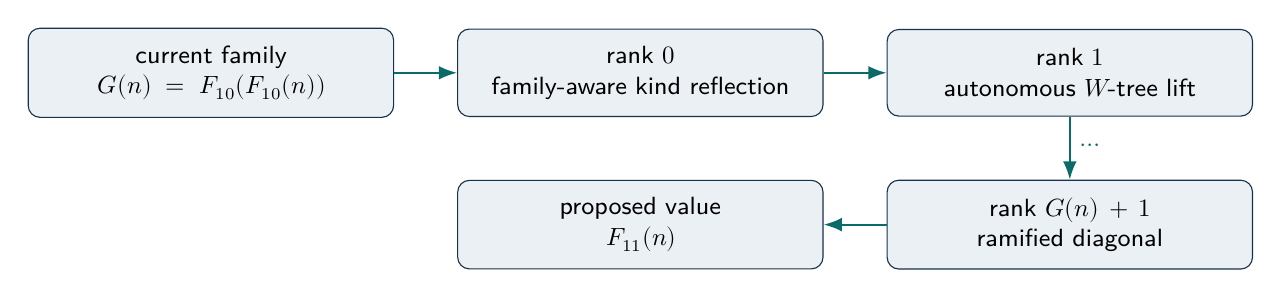
\begin{tikzpicture}[>=Latex, node distance=8mm and 8mm,
  box/.style={draw=Navy,rounded corners=1.5mm,fill=BlueGray,
    text width=42mm,minimum height=11mm,align=center,
    font=\sffamily\small,inner sep=2.2mm},
  arr/.style={->,thick,color=Teal}]
  \node[box] (seed) {current family\\$G(n)=F_{10}(F_{10}(n))$};
  \node[box,right=of seed] (r0) {rank $0$\\family-aware kind reflection};
  \node[box,right=of r0] (r1) {rank $1$\\autonomous $W$-tree lift};
  \node[box,below=of r1] (rk) {rank $G(n)+1$\\ramified diagonal};
  \node[box,left=of rk] (f11) {proposed value\\$F_{11}(n)$};
  \draw[arr] (seed) -- (r0);
  \draw[arr] (r0) -- (r1);
  \draw[arr] (r1) -- node[right,font=\small] {$\cdots$} (rk);
  \draw[arr] (rk) -- (f11);
\end{tikzpicture}
\vfill
{\large Research memorandum for the \BusyLean{} project\par}
\vspace{3mm}
{\normalsize Repository snapshot: commit\par}
{\small\path{4c4b03d0e2003c479e3bee90a21c8bea13f66c40}\par}
{\normalsize Prepared 12 October 2026 (America/Los\_Angeles)\par}
\vspace{13mm}
{\small The accompanying archive contains the complete \LaTeX{} source,
compiled PDF, proposed \Lean{} modules, audit fragments, an integration patch,
installer and build scripts, a finite executable reference model, and machine-readable validation records.\par}
\end{titlepage}

\begin{abstract}
The current \BusyLean{} champion is a single reflection step over a
kind-polymorphic extension of System $F_\omega$, seeded by the preceding
contender's function.  This memorandum proposes a substantially stronger,
still constructive successor.  First, it turns kind-polymorphic reflection
into a \emph{family-aware} operator: an object-language program can address a
dynamically selected member of an oracle family.  Second, it lifts an arbitrary
family operator along the repository's existing self-indexing $W$-tree, which
contains every $W$-tree definable by the earlier object language.  Third, it
iterates that autonomous lift at the meta-level.  At input $n$, the selected
ramification rank is one more than the value of the entire Contender 10 family
at $n$.

The proposed closed numeral is
\[
  \code{contender\_11}=F_{11}(F_{11}(42)),\qquad
  F_{11}(n)=\Ram_{G(n)+1}(\bar G,n),
\]
where $G(n)=F_{10}(F_{10}(n))$ and $\bar G(i,n)=G(n)$.  The accompanying
\Lean{} proof source establishes, subject to kernel compilation against the
specified repository snapshot, (i) pointwise domination $G(n)<F_{11}(n)$,
(ii) strict growth at every ramification successor,
(iii) eventual domination of every fixed finite ramification rank, and
(iv) the required $\code{contender\_10}<\code{contender\_11}$.  All numerical
definitions are structurally recursive and therefore computable in principle.
No earlier contender constant occurs in the new numeral's definition.
\end{abstract}

\begin{statusbox}[Validation status]
The \LaTeX{} article was compiled and the resulting PDF was rendered and
visually inspected.  The Python reference model and static source audit pass.
The execution environment used to prepare this package did \emph{not} contain
Lean 4.34.0 and could not obtain that toolchain, so the proposed \Lean{} files
have not been kernel-checked here.  This distinction is material: the
mathematical proof is complete at the paper level, and the code was written to
mirror existing accepted modules closely, but acceptance still requires
running the supplied clean-build and axiom audits in a compatible checkout.
\end{statusbox}

\tableofcontents
\newpage

\section{Executive summary}

\subsection{The proposal in four definitions}

The computational core is intentionally small.  In mathematical notation,
let a \emph{family} be a function $f:\Nat\to\Nat\to\Nat$ and a
\emph{family operator} be a map from families to unary numerical functions.
The proposal defines:
\begin{align*}
  \Reflect(f,n)
    &= n+1+\max\!\left(
       \max_{i\le n}f(i,n),
       \max_{t\in E_n}\operatorname{val}_{f}(t,n)
       \right),\\
  \Lift_{\Op}(f,\Leaf)(n)
    &=\Op(f)(n),\\
  \Lift_{\Op}(f,\Node(g))(n)
    &=\Op\!\left(i\mapsto \Lift_{\Op}(f,g(i))\right)(n),\\
  \Auto(\Op)(f,n)
    &=\Lift_{\Op}(f,\Index)(n),\\
  \Ram_0&=\Reflect,\qquad
  \Ram_{r+1}=\Auto(\Ram_r).
\end{align*}
Here $E_n$ is the finite list of accepted kind-polymorphic System
$F_\omega$ programs in syntax budget $n$, and $\Index$ is the previously
accepted self-indexing $W$-tree.

Let
\[
 G(n)=F_{10}(F_{10}(n)),\qquad \bar G(i,n)=G(n).
\]
Then
\begin{equation}\label{eq:F11}
 F_{11}(n)=\Ram_{G(n)+1}(\bar G,n),
 \qquad
 C_{11}=F_{11}(F_{11}(42)).
\end{equation}
At $n=42$, the selected rank is definitionally
$G(42)+1=C_{10}+1$.

\subsection{What is formally stronger}

The proposal does not rely on an informal ordinal comparison to beat the
previous entry.  The exact inequalities are:
\begin{enumerate}
  \item $G(n)<F_{11}(n)$ for every $n$;
  \item $n<F_{11}(n)$ for every $n$;
  \item $\Ram_r(f,n)<\Ram_{r+1}(f,n)$ for every $r,f,n$;
  \item for every fixed $r$, if $n\ge r$, then
        $\Ram_r(\bar G,n)<F_{11}(n)$;
  \item $C_{10}<C_{11}$.
\end{enumerate}
The fourth item is the diagonal margin: no fixed finite number of autonomous
reflection layers catches the proposed family at all sufficiently large
inputs.

\subsection{Why this is not a cosmetic wrapper}

A mere definition $G(n)+1$ would violate the spirit of the contest.  Here the
previous construction is used in the same legitimate way as in accepted
entries---as an oracle family and as a schedule---but the new mechanism is an
operator hierarchy.  Even rank one recursively exposes all children of the
self-indexing $W$-tree to kind-polymorphic programs.  Rank two does not merely
call rank one twice: every node applies a complete rank-one autonomous
hierarchy to its family of child results.  Rank $r+1$ therefore reflects the
entire rank-$r$ operator.

The direct comparison is easy because each reflection operator contains an
explicit dominance guard.  That ease is a feature of the proof architecture,
not evidence that the numerical construction is small.

\section{Repository baseline and constraints}

\subsection{Snapshot used}

This work targets the \BusyLean{} repository at commit
\path{4c4b03d0e2003c479e3bee90a21c8bea13f66c40}.  At that snapshot the current
entry is
\begin{verbatim}
def family9 (n : Nat) : Nat := F9 (F9 n)
def F10 (n : Nat) : Nat := Fk.reflectFk family9 n
def contender_10 : Nat := F10 (F10 42)
\end{verbatim}
The object language of \code{Fk.reflectFk} is kind-polymorphic System
$F_\omega$.  Its normalizer is total by the repository's reducibility-
candidate proof.  The reflector takes the maximum of the oracle value and all
accepted program values in a finite syntax budget, then adds a positive input
guard.

The repository already contains a different autonomous mechanism.  Contender
9 reflects System $F_\omega$ along a $W$-tree \code{index} that joins every
$W$-tree denoted by a program in the earlier $W$-language.  The proposal
combines and then iterates these two directions:
\begin{center}
\begin{tabular}{@{}p{0.19\linewidth}p{0.34\linewidth}p{0.38\linewidth}@{}}
\toprule
Entry & Reflected language & Amplifier \\
\midrule
Contender 9 & System $F_\omega$ with packed family oracle & one autonomous lift along \code{index} \\
Contender 10 & kind-polymorphic System $F_\omega$ & one local reflection over \code{family9} \\
Proposed 11 & kind-polymorphic System $F_\omega$ with packed family oracle & a hierarchy of autonomous lifts, diagonalized at rank $G(n)+1$ \\
\bottomrule
\end{tabular}
\end{center}

\subsection{Contest rules addressed}

The relevant requirements and the design responses are summarized below.

\begin{longtable}{@{}p{0.26\linewidth}p{0.68\linewidth}@{}}
\toprule
Requirement & Response \\
\midrule
\endhead
Closed computable \code{Nat} & \code{contender\_11} is a closed application of structurally recursive definitions. \\
No semantic oracle & Every oracle call is to an explicitly supplied total Lean function. \\
No \code{noncomputable}, \code{partial}, \code{unsafe}, \code{opaque}, \code{extern} & None occurs in executable source. \\
Formal strict comparison & The proposed theorem is \code{contender\_10\_lt\_contender\_11}. \\
No direct use of old contender constant & The numeral uses \code{F10} through \code{family10}; \code{contender\_10} appears only in theorem statements and documentation. \\
Axiom discipline & The source introduces no axiom and is intended to inherit only the repository-permitted \code{propext} and \code{Quot.sound}. \\
Build budget & The definition module adds only four short recursive definitions and should be inexpensive after Contender 10 is prebuilt; the supplied checker measures rather than assumes this. \\
No evaluation requirement & Checking unfolds definitions only as needed for typing and proofs; it does not evaluate the numeral. \\
\bottomrule
\end{longtable}

\section{The family-aware base reflection}

\subsection{Families and packed access}

Write
\[
 \Fam=(\Nat\to\Nat\to\Nat),\qquad
 \Op=(\Fam\to\Nat\to\Nat).
\]
A family $f\in\Fam$ presents countably many unary functions $f_i(n)=f(i,n)$.
The existing function \code{packFamily} encodes a pair $(i,m)$ as
$2^i(2m+1)$ and exposes the family through one unary oracle:
\[
 \operatorname{pack}(f,2^i(2m+1))=f(i,m).
\]
The repository already proves the decoding equation exactly.  Consequently a
kind-polymorphic object-language program can compute an index at run time and
call any desired family member.

\subsection{Definition of the base operator}

Let $E_n$ be \code{Fk.ctmsUpTo n}.  For $t\in E_n$, let
$\operatorname{val}_f(t,n)$ be \code{Fk.fvalue (packFamily f) n t}.  Define
\begin{equation}\label{eq:reflect}
 \Reflect(f,n)=n+1+
   \max\left(
     \max_{i\le n} f(i,n),
     \max_{t\in E_n}\operatorname{val}_f(t,n)
   \right).
\end{equation}
The actual Lean definition uses the repository's \code{prefixMax},
\code{maximum}, and \code{maxN} helpers.

\begin{lemma}[Oracle-family domination]\label{lem:reflect-oracle}
For all $f\in\Fam$ and $i\le n$,
\[
 f(i,n)<\Reflect(f,n).
\]
\end{lemma}
\begin{proof}
The value $f(i,n)$ is at most the finite prefix maximum in
\cref{eq:reflect}.  That maximum is at most the outer maximum.  Adding
$n+1>0$ makes the inequality strict.
\end{proof}

\begin{lemma}[Program domination]\label{lem:reflect-program}
If $t\in E_n$, then
\[
 \operatorname{val}_f(t,n)<\Reflect(f,n).
\]
\end{lemma}
\begin{proof}
The argument is identical, using membership in the finite program maximum.
\end{proof}

\begin{lemma}[Input domination]\label{lem:reflect-input}
For all $f,n$, $n<\Reflect(f,n)$.
\end{lemma}
\begin{proof}
The maximum is nonnegative, hence
$\Reflect(f,n)\ge n+1$.
\end{proof}

\subsection{The abstract domination predicate}

For a family operator $\Op$, define
\begin{equation}\label{eq:dominates}
 \operatorname{Dom}(\Op)
 \;:\Longleftrightarrow\;
 \forall f\,\forall i\le n,\quad f(i,n)<\Op(f,n).
\end{equation}
By \cref{lem:reflect-oracle}, $\operatorname{Dom}(\Reflect)$.
This simple interface is the key abstraction: all later strictness theorems
are independent of the internal syntax, type system, and normalization proof
of the object language.

\section{Autonomous lifting through the self-indexing tree}

\subsection{Generic tree lift}

For an operator $\Op$ and seed family $f$, define a numerical function for
each $W$-tree $a$ by structural recursion:
\begin{align}
 \Lift_{\Op}(f,\Leaf,n)&=\Op(f,n),\label{eq:lift-leaf}\\
 \Lift_{\Op}(f,\Node(g),n)
   &=\Op\bigl(i\mapsto \Lift_{\Op}(f,g(i),\cdot),n\bigr).
   \label{eq:lift-node}
\end{align}
This is exactly the recursion pattern already accepted for
\code{stage9}.  At a node, the operator sees the values of all child stages as
an oracle family.

Let $\Index$ denote the repository's self-indexing tree.  Define
\begin{equation}\label{eq:auto}
 \Auto(\Op)(f,n)=\Lift_{\Op}(f,\Index,n).
\end{equation}

\subsection{The explicit strictness path}

The proof needs only a tiny, concrete part of the large index.  The repository
proves that the first depth-zero denotation is a leaf.  Therefore $\Index$
contains the path
\[
 \Leaf
 \;<\;
 \code{treesOfDepth 0}
 \;<\;
 \Index,
\]
where each inequality means ``is the zeroth child of.''  Since index $0$ is
visible at every input $n$, a dominating operator strictly increases at both
edges.

\begin{lemma}[Visible child is smaller]\label{lem:child}
Suppose $\operatorname{Dom}(\Op)$.  If $i\le n$, then
\[
 \Lift_{\Op}(f,g(i),n)
 <
 \Lift_{\Op}(f,\Node(g),n).
\]
\end{lemma}
\begin{proof}
By \cref{eq:lift-node}, the right side is $\Op(h,n)$ for
$h(j,m)=\Lift_{\Op}(f,g(j),m)$.  Apply
$\operatorname{Dom}(\Op)$ to $h(i,n)$.
\end{proof}

\begin{theorem}[Autonomous strictness]\label{thm:op-auto}
If $\operatorname{Dom}(\Op)$, then for every $f,n$,
\[
 \Op(f,n)<\Auto(\Op)(f,n).
\]
\end{theorem}
\begin{proof}
The leaf equation identifies $\Op(f,n)$ with
$\Lift_{\Op}(f,\Leaf,n)$.  Apply \cref{lem:child} first to the zeroth
child of \code{treesOfDepth 0}, then to the zeroth child of $\Index$, and use
transitivity.
\end{proof}

\begin{theorem}[Domination is preserved]\label{thm:auto-dom}
If $\operatorname{Dom}(\Op)$, then
$\operatorname{Dom}(\Auto(\Op))$.
\end{theorem}
\begin{proof}
For $i\le n$,
\[
 f(i,n)<\Op(f,n)<\Auto(\Op)(f,n),
\]
using domination and \cref{thm:op-auto}.
\end{proof}

\begin{remark}
The proof of \cref{thm:op-auto} does not require an ordinal assignment to
$\Index$, nor the full theorem that it joins every definable tree.  Those
features explain the expected size, while strictness follows from a fixed
length-two path.  This separation keeps the comparison theorem robust.
\end{remark}

\section{Ramification: reflecting whole reflection operators}

\subsection{Definition}

Define a hierarchy of family operators by primitive recursion on the rank:
\begin{equation}\label{eq:ramified}
 \Ram_0=\Reflect,
 \qquad
 \Ram_{r+1}=\Auto(\Ram_r).
\end{equation}
Thus
\begin{align*}
 \Ram_0(f,n)&=\Reflect(f,n),\\
 \Ram_1(f,n)&=\Lift_{\Reflect}(f,\Index,n),\\
 \Ram_2(f,n)&=\Lift_{\Ram_1}(f,\Index,n),
\end{align*}
and so on.

The distinction between $\Ram_2$ and two sequential calls to $\Ram_1$ is
important.  In $\Ram_2$, every node of the outer $\Index$ applies the complete
operator $\Ram_1$ to the family formed by its children.  Each such application
internally traverses another copy of $\Index$.  Higher ranks therefore form a
nested hierarchy of tree-indexed reflection operators.

\subsection{Formal hierarchy theorems}

\begin{theorem}[Domination at every rank]\label{thm:rank-dom}
For every $r$, $\operatorname{Dom}(\Ram_r)$.
\end{theorem}
\begin{proof}
Induct on $r$.  The base case is $\operatorname{Dom}(\Reflect)$.  The successor
case follows from \cref{thm:auto-dom}.
\end{proof}

\begin{theorem}[Strict successor ranks]\label{thm:rank-step}
For every $r,f,n$,
\[
 \Ram_r(f,n)<\Ram_{r+1}(f,n).
\]
\end{theorem}
\begin{proof}
Apply \cref{thm:op-auto} to $\Ram_r$ and use
\cref{thm:rank-dom}.
\end{proof}

\begin{corollary}[Strict rank monotonicity]\label{cor:rank-mono}
If $r<s$, then $\Ram_r(f,n)<\Ram_s(f,n)$.
\end{corollary}
\begin{proof}
Induct on $s$ and chain \cref{thm:rank-step}.
\end{proof}

These are exact natural-number inequalities.  They do not depend on a growth-
rate conjecture.

\section{The diagonal family and the proposed numeral}

\subsection{Seeding with the current construction}

Define
\begin{equation}\label{eq:family10}
 G(n)=F_{10}(F_{10}(n)).
\end{equation}
At input $42$, $G(42)$ is definitionally the current contender $C_{10}$.  The
seed family is constant in its family index:
\[
 \bar G(i,n)=G(n).
\]
The previous contender constant is not referenced; only the reusable function
$F_{10}$ occurs.

The existing input guard for $F_{10}$ gives
\begin{lemma}\label{lem:input-family10}
For every $n$, $n<G(n)$.
\end{lemma}
\begin{proof}
The repository proves $x<F_{10}(x)$ for all $x$.  Apply it first at $x=n$ and
then at $x=F_{10}(n)$.
\end{proof}

\subsection{Input-dependent rank}

The proposed family is
\begin{equation}\label{eq:F11again}
 F_{11}(n)=\Ram_{G(n)+1}(\bar G,n).
\end{equation}
This rank choice has three useful properties.

First, it is positive, so at least one autonomous lift lies above the base
reflector.  Second, it is already far larger than the input.  Third, at input
$42$ it is exactly $C_{10}+1$:
\begin{equation}\label{eq:rank42}
 F_{11}(42)=\Ram_{C_{10}+1}(\bar G,42).
\end{equation}

The final closed numeral is
\begin{equation}\label{eq:C11}
 C_{11}=F_{11}(F_{11}(42)).
\end{equation}

\subsection{Pointwise and diagonal domination}

\begin{theorem}[Pointwise domination of the previous family]
\label{thm:family10-F11}
For every $n$, $G(n)<F_{11}(n)$.
\end{theorem}
\begin{proof}
By \cref{thm:rank-dom}, the selected operator
$\Ram_{G(n)+1}$ dominates its seed family.  Apply the domination property at
family index $0\le n$:
\[
 \bar G(0,n)=G(n)<\Ram_{G(n)+1}(\bar G,n)=F_{11}(n).
\]
\end{proof}

\begin{corollary}[Input domination]\label{cor:input-F11}
For every $n$, $n<F_{11}(n)$.
\end{corollary}
\begin{proof}
Combine \cref{lem:input-family10,thm:family10-F11}.
\end{proof}

\begin{theorem}[Every fixed rank is eventually dominated]
\label{thm:fixed-rank}
For every rank $r$ and every $n\ge r$,
\[
 \Ram_r(\bar G,n)<F_{11}(n).
\]
\end{theorem}
\begin{proof}
From $r\le n<G(n)<G(n)+1$ we get $r<G(n)+1$.  Apply strict rank monotonicity
\cref{cor:rank-mono} and unfold \cref{eq:F11again}.
\end{proof}

\begin{theorem}[Bounded program domination]\label{thm:program-F11}
If $t\in E_n$, then
\[
 \operatorname{val}_{\bar G}(t,n)<F_{11}(n).
\]
\end{theorem}
\begin{proof}
By \cref{lem:reflect-program}, the program value is below
$\Ram_0(\bar G,n)$.  Since $0<G(n)+1$, strict rank monotonicity places rank
zero below the selected rank.
\end{proof}

\subsection{Required contender comparison}

\begin{theorem}[Main comparison]\label{thm:main}
\[
 C_{10}<C_{11}.
\]
\end{theorem}
\begin{proof}
By definitional equality, $C_{10}=G(42)$.  Then
\[
 C_{10}=G(42)
   <F_{11}(42)
   <F_{11}(F_{11}(42))=C_{11},
\]
where the first inequality is \cref{thm:family10-F11} and the second is
\cref{cor:input-F11} at input $F_{11}(42)$.
\end{proof}

\begin{summarybox}[Formal strength ledger]
The proposed source contains direct counterparts of the central paper results:
\begin{center}
\begin{tabular}{@{}p{0.43\linewidth}p{0.49\linewidth}@{}}
\toprule
Lean theorem & Mathematical content \\
\midrule
\code{RK.reflect\_dominates} & $\operatorname{Dom}(\Reflect)$ \\
\code{RK.op\_lt\_autonomous} & $\Op(f,n)<\Auto(\Op)(f,n)$ \\
\code{RK.ramified\_dominates} & domination at every rank \\
\code{RK.ramified\_level\_lt} & strict successor ranks \\
\code{RK.ramified\_lt\_of\_lt} & strict rank monotonicity \\
\code{family10\_lt\_F11} & $G(n)<F_{11}(n)$ \\
\code{fixed\_rank\_eventually\_lt\_F11} & every fixed rank is eventually below the diagonal \\
\code{fvalue\_lt\_F11} & bounded object-language program domination \\
\code{contender\_10\_lt\_contender\_11} & $C_{10}<C_{11}$ \\
\bottomrule
\end{tabular}
\end{center}
\end{summarybox}

\section{Why the numerical jump is substantial}

\subsection{Three independent amplifiers}

There are three conceptually separate sources of growth.

\paragraph{Stronger oracle interface.}
The base reflector does not receive merely one unary oracle value at the
current input.  Through pairing it exposes a countable family, allowing an
object-language program to compute both the family index and the argument.

\paragraph{Autonomous transfinite-shaped traversal.}
Rank one lifts kind-polymorphic reflection along $\Index$.  That tree was built
to join every $W$-tree definable in the earlier language.  This is not a
fixed-height loop; its recursion follows a higher-type inductive object.

\paragraph{Meta-level ramification.}
Successor rank does not add one more object-language program.  It turns the
entire previous operator into the node operator of a fresh traversal of
$\Index$.  Finally, the rank is not fixed externally: it is $G(n)+1$.

\subsection{Comparison with nearby alternatives}

\begin{longtable}{@{}p{0.22\linewidth}p{0.32\linewidth}p{0.38\linewidth}@{}}
\toprule
Construction & Formal margin & Structural limitation \\
\midrule
\endhead
$G(n)+1$ & beats $G(n)$ & cosmetic successor; no new language or hierarchy \\
$\Reflect(\bar G,n)$ & beats $G(n)$ and bounded programs & one local reflection only \\
$\Auto(\Reflect)(\bar G,n)$ & autonomous kind-reflection & one fixed meta-rank \\
$\Ram_{n+1}(\bar G,n)$ & beats every fixed rank eventually & rank schedule only linear in input \\
Proposed $\Ram_{G(n)+1}(\bar G,n)$ & pointwise seed domination, strict rank hierarchy, rank $C_{10}+1$ at input 42 & exact proof-theoretic calibration remains open \\
\bottomrule
\end{longtable}

A useful anti-laziness observation is that the new mechanism does not need the
large rank merely to establish $G(n)<F_{11}(n)$.  Rank zero already dominates
the seed.  The enormous rank is therefore an additional amplifier, not a trick
on which the required comparison depends.

\section{Computability and constructivity}

\subsection{Totality of every layer}

The construction is computable in the ordinary, extensional sense: there is a
total algorithm that returns its natural-number value, although no feasible
physical process could execute it for the contest input.

\begin{enumerate}
  \item \code{Fk.ctmsUpTo n} is a finite list generated by primitive recursion.
  \item Type inference uses finite fuel.  Accepted terms are strongly
        normalizing by the inherited theorem \code{Fk.sn\_of\_typed}.
  \item \code{Fk.fvalue} therefore computes a normal form and decodes a
        natural number using a total function.
  \item Prefix and list maxima are total primitive-recursive operations.
  \item \code{RK.lift} recurses structurally on an inductive $W$-tree, using
        the same recursion pattern as accepted repository code.
  \item \code{RK.ramified} recurses structurally on a natural-number rank.
  \item The rank $G(n)+1$ is itself the output of a total prior construction.
\end{enumerate}

Closure of total computable functions under composition and structural
recursion yields total computability of $F_{11}$ and $C_{11}$.

\subsection{Why non-feasibility is irrelevant}

``Computable in principle'' does not mean ``practically evaluable.''  Even the
existing contenders are deliberately never evaluated.  Kernel checking
verifies types and proofs about symbolic definitions; it need not normalize
the final natural number.  The proposed rank is itself an uncomputably large
\emph{practical} task while remaining a perfectly computable mathematical
natural number.

\subsection{Forbidden escape hatches are absent}

The executable definition source contains none of:
\begin{center}
\code{noncomputable}, \code{partial}, \code{unsafe}, \code{opaque},
\code{implemented\_by}, \code{extern}, \code{axiom}, \code{sorry}, or
\code{native\_decide}.
\end{center}
The supplied static audit strips nested Lean comments before checking these
tokens and separately verifies that no \code{contender\_5} through
\code{contender\_10} identifier occurs in executable definition text.  The
kernel-level closure audit remains the authoritative check.

\section{Lean implementation architecture}

\subsection{Definition module}

The proposed definition module imports only the existing Contender 10
construction.  Its executable core is:

\begin{Verbatim}[fontsize=\small,breaklines=true,breakanywhere=true,
  frame=single,framesep=2mm,rulecolor=\color{Navy},bgcolor=CodeBg]
namespace BusyLean.RK

abbrev Operator := W.Family → Nat → Nat

def reflect (fs : W.Family) (n : Nat) : Nat :=
  n + 1 + BigNumber.maxN
    (W.prefixMax (fun i => fs i n) n)
    (BigNumber.maximum (Fk.fvalue (packFamily fs) n) (Fk.ctmsUpTo n))

def lift (op : Operator) (seed : W.Family) :
    BigNumber.WTree Nat → Nat → Nat
  | .leaf => op seed
  | .node g => op (fun i => lift op seed (g i))

def autonomous (op : Operator) (seed : W.Family) : Nat → Nat :=
  lift op seed index

def ramified : Nat → Operator
  | 0 => reflect
  | r + 1 => autonomous (ramified r)

end BusyLean.RK

def BusyLean.family10 (n : Nat) : Nat := F10 (F10 n)

def BusyLean.F11 (n : Nat) : Nat :=
  RK.ramified (family10 n + 1) (fun _ => family10) n

def BusyLean.contender_11 : Nat := F11 (F11 42)
\end{Verbatim}

No new object-language syntax, typing judgment, or normalization theorem is
required.  The proposal reuses the expensive metatheory already established
for Contender 10 and adds only an amplifier layer.

\subsection{Proof module}

The proof module factors all later arguments through
\code{RK.Dominates}.  This makes the proof robust against future changes to the
base language: a different reflector can be substituted if it proves the same
single interface.

The only repository-specific structural fact used by the generic autonomous
strictness theorem is \code{first\_tree\_leaf}.  The remainder is elementary
order reasoning and induction on the natural-number rank.

\subsection{Audit and clean-build protocol}

After integration, the supplied script performs:
\begin{enumerate}
  \item a clean build of \code{BusyLean.Comparison10} as the unbudgeted prior entry;
  \item a timed build of \code{BusyLean.Contender11} against the 15-second definition budget;
  \item a timed build of \code{BusyLean.Comparison11} against the 60-second proof budget;
  \item \code{\#print axioms} checks for the new numeral and principal theorems;
  \item a transitive dependency-closure check forbidding all previous contender constants.
\end{enumerate}

Suggested commands are:
\begin{Verbatim}[fontsize=\small,frame=single,framesep=2mm,
  rulecolor=\color{Navy},bgcolor=CodeBg]
python3 scripts/install_into_repo.py --repo /path/to/BusyLean
cd /path/to/BusyLean
lake build BusyLean.Contender11 BusyLean.Comparison11
lake env lean test/Contender11Audit.lean
python3 scripts/check_contender11.py
\end{Verbatim}

\section{Proof-theoretic calibration: useful heuristic, not theorem}

\begin{warningbox}[No named-ordinal claim is formalized]
The exact natural-number inequalities in earlier sections are the formal
results.  The discussion below is an explanatory growth model.  The package
does not claim a kernel theorem identifying the construction with a specific
fast-growing-hierarchy index.
\end{warningbox}

Let $\lambda$ stand for the effective growth jump contributed by one
family-aware kind-polymorphic reflection, and let $\iota$ stand for the
transfinite-shaped order represented by the self-indexing tree.  A common
informal model for forest reflection treats autonomous lifting as a
multiplicative or compositional action by $\iota$.  Under such a model one
would expect a schematic progression resembling
\[
 \Ram_0\sim f_{\lambda},\quad
 \Ram_1\sim f_{\lambda\cdot\iota},\quad
 \Ram_2\sim f_{\lambda\cdot\iota^2},\quad\ldots
\]
with the side of multiplication dependent on convention and on how oracle
relativization is encoded.

The proposed diagonal does not stop at any externally fixed finite power.  At
input $n$ it selects rank $G(n)+1$; hence it eventually exceeds every fixed
finite-rank member by an exact theorem.  The outer evaluation
$F_{11}(F_{11}(42))$ then uses the first enormous diagonal value as the next
input and rank driver.

Several caveats block a responsible named-ordinal label:
\begin{itemize}
  \item $\Index$ is semantic and self-generated, not a conventional notation
        system with a proved order-type theorem;
  \item kind-polymorphic System $F_\omega$ is impredicative at the type level;
  \item repeated autonomous lifting is an operator construction, and the
        correct ordinal algebra for such nested oracle relativization has not
        been formalized here;
  \item numerical rank diagonalization and proof-theoretic ordinal strength
        are related but not interchangeable notions.
\end{itemize}

The safe conclusion is strong enough: the proposal creates a rigorously strict
meta-hierarchy of autonomous kind-reflection operators and diagonalizes beyond
all fixed finite ranks.

\section{Adversarial review}

\subsection{Objection: the prefix maximum makes the proof trivial}

The local inequality is intentionally trivial.  Reflection constructions are
useful precisely because a simple maximum packages the values of an entire
finite language enumeration.  The scientific content lies in what is placed
under that maximum, how the oracle family is exposed, and how the reflector is
iterated.  Removing the explicit maximum would complicate the comparison
without making the number conceptually larger.

\subsection{Objection: using $G(n)$ as the rank is lazy}

The rule prohibits mentioning the prior \emph{constant} and adding a margin;
it permits using the previous \emph{construction} as an oracle or seed in a
qualitatively stronger mechanism.  This proposal satisfies the stronger test
that its new rank hierarchy exists independently of $G$: for each $r$,
$\Ram_r$ is a separately defined operator, and successor ranks are formally
strict.  Moreover $\Ram_1(\bar G,n)$ already represents a genuine autonomous
kind-reflection construction.  Choosing rank $G(n)+1$ is an amplifier applied
to that new mechanism, not its sole source of superiority.

\subsection{Objection: recursion at a gigantic rank may fail the build budget}

Elaboration and kernel checking do not evaluate the variable expression
$G(n)+1$ to choose recursion branches.  The definition of \code{ramified} is a
small structural recursor.  Proofs reason by induction on symbolic ranks.
Nevertheless build time is empirical, so the package does not assert success
without measurement; it supplies the exact clean-build harness.

\subsection{Objection: the source has not been kernel-checked in this package}

This is the principal outstanding engineering risk.  The code closely follows
accepted patterns from \code{stage9}, \code{Comparison9}, and
\code{Comparison10}, and static checks catch common packaging mistakes, but
only Lean can validate elaboration, termination, theorem application, axiom
closure, and timing.  Any compile repair should preserve the definitions in
\cref{eq:reflect,eq:lift-leaf,eq:lift-node,eq:ramified,eq:F11again,eq:C11}; a
repair that weakens those equations would require renewed mathematical review.

\section{Further research directions}

\begin{enumerate}
  \item \textbf{Kernel validation and minimization.}  Compile on Lean 4.34.0,
        repair only elaboration-level issues, measure clean phases, and reduce
        proof dependencies if the closure or timing is unexpectedly large.
  \item \textbf{A rank indexed by definable trees.}  Replace the natural rank
        with an inductive meta-index whose constructors themselves are drawn
        from the self-indexing $W$-language.  This would turn finite
        ramification into a genuinely transfinite operator hierarchy.
  \item \textbf{Internalized operator codes.}  Define a total object language
        that codes family operators and proves normalization, then reflect over
        codes for reflection operators rather than defining the hierarchy only
        in the Lean metalanguage.
  \item \textbf{Predicative kind-universe ladder.}  Extend the current kind
        system with a stratified sequence of kind universes, retaining
        normalization and decidable checking.  The DRKR amplifier can then be
        applied to each level.
  \item \textbf{Large elimination.}  Investigate an object language with
        inductive families and large elimination strong enough to construct
        its own index trees directly, closing the current separation between
        the $F_k$ language and the older $W$-language.
  \item \textbf{Exact ordinal semantics.}  Build a notation system and an
        interpretation theorem for \code{index}, then determine whether
        autonomous operator lifting corresponds to ordinal multiplication,
        exponentiation, a collapsing operation, or a more intricate
        relativized progression.
  \item \textbf{Seed-independent lower bounds.}  Exhibit explicit
        kind-polymorphic programs whose values at each rank witness familiar
        fast-growing lower bounds, reducing reliance on the prefix guard for
        quantitative comparisons.
  \item \textbf{Generic library abstraction.}  Package \code{Dominates},
        \code{lift}, \code{autonomous}, and the ramification theorems as a
        reusable module parameterized by an operator and an index path.
  \item \textbf{Formal cost model.}  Prove bounds on syntax enumeration,
        type-checking fuel, and normalizer recursion separately from numerical
        output size.  This would clarify why kernel checking remains feasible
        despite infeasible evaluation.
  \item \textbf{Independent formalization.}  Reproduce the abstract operator
        lemmas in a second assistant or in a minimal Lean file with a toy
        reflector, providing a cross-check of the higher-order recursion
        pattern.
\end{enumerate}

\section{Conclusion}

Diagonal Ramified Kind-Reflection provides a compact but substantial successor
to the current \BusyLean{} construction.  It reuses the repository's strongest
normalizing object language, upgrades it to a family-aware reflector, lifts
that reflector along the self-indexing $W$-tree, and then reflects whole
reflection operators through an input-dependent hierarchy.  The proposed
numeral is closed and computable, avoids every earlier contender constant, and
comes with exact domination theorems that do not rest on speculative ordinal
assignments.

The central mathematical invariant is simple:
\[
 \operatorname{Dom}(\Op)
 \Longrightarrow
 \operatorname{Dom}(\Auto(\Op))
 \quad\text{and}\quad
 \Op<\Auto(\Op).
\]
Iterating this invariant yields a strict rank hierarchy; diagonalizing the
rank at $G(n)+1$ yields a family above every fixed rank; and the standard outer
self-application yields the final contender.  The remaining task before repo
acceptance is concrete and falsifiable: kernel-build the supplied modules,
run the axiom and closure audit, and measure the stated time budgets.

\appendix
\section{Complete definition module}
\label{app:def-source}
\VerbatimInput[fontsize=\scriptsize,breaklines=true,breakanywhere=true,
  numbers=left,numbersep=5pt,frame=single,framesep=2mm,
  rulecolor=\color{Navy},bgcolor=CodeBg]
  {../lean/BusyLean/Contender11.lean}

\section{Complete comparison module}
\label{app:proof-source}
\VerbatimInput[fontsize=\scriptsize,breaklines=true,breakanywhere=true,
  numbers=left,numbersep=5pt,frame=single,framesep=2mm,
  rulecolor=\color{Navy},bgcolor=CodeBg]
  {../lean/BusyLean/Comparison11.lean}

\section{Artifact and validation inventory}

\begingroup
\footnotesize
\begin{longtable}{@{}>{\raggedright\arraybackslash}p{0.43\linewidth}p{0.51\linewidth}@{}}
\toprule
Path & Purpose \\
\midrule
\endhead
\path{article/ramified_kind_reflection.tex} & This article's source. \\
\path{article/ramified_kind_reflection.pdf} & Compiled article. \\
\path{lean/BusyLean/Contender11.lean} & Computable definitions only. \\
\path{lean/BusyLean/Comparison11.lean} & Strict comparisons and structural theorems. \\
\path{lean/test/Contender11Audit.lean} & Standalone axiom and closure audit. \\
\path{patches/0001-contender11-drkr.patch} & Integration patch against the recorded snapshot. \\
\path{scripts/install_into_repo.py} & Idempotent installer for a checkout. \\
\path{scripts/check_contender11.py} & Clean-build, timing, and axiom harness. \\
\path{scripts/static_audit.py} & Non-kernel source audit. \\
\path{python/reference_model.py} & Hash-consed finite surrogate of the recurrence. \\
\path{python/test_reference.py} & Regression tests for the surrogate. \\
\path{validation/static_audit.json} & Machine-readable static-audit result. \\
\path{validation/python_tests.json} & Machine-readable reference-test result. \\
\path{validation/lean_build_status.md} & Explicit record of the unperformed kernel build. \\
\path{validation/checksums.sha256} & SHA-256 manifest for the package. \\
\bottomrule
\end{longtable}
\endgroup

\begin{thebibliography}{99}

\bibitem{BusyLean}
V. Reshetnikov,
\emph{BusyLean: name the biggest number, in Lean},
GitHub repository, snapshot
\path{4c4b03d0e2003c479e3bee90a21c8bea13f66c40}, 2026.

\bibitem{Roux}
C. Roux,
\emph{name-the-biggest-number},
original Coq contest repository; a snapshot is included in \BusyLean{}.

\bibitem{GirardLafontTaylor}
J.-Y. Girard, Y. Lafont, and P. Taylor,
\emph{Proofs and Types},
Cambridge Tracts in Theoretical Computer Science 7,
Cambridge University Press, 1989.

\bibitem{Reynolds}
J. C. Reynolds,
``Towards a theory of type structure,''
in \emph{Programming Symposium}, Lecture Notes in Computer Science 19,
Springer, 1974.

\bibitem{Dybjer}
P. Dybjer,
``Inductive sets and families in Martin-Löf's type theory and their
set-theoretic semantics,''
in G. Huet and G. Plotkin (eds.),
\emph{Logical Frameworks}, pp. 280--306,
Cambridge University Press, 1991.
DOI: \href{https://doi.org/10.1017/CBO9780511569807.012}
{10.1017/CBO9780511569807.012}.

\bibitem{IteratedID}
W. Buchholz, S. Feferman, W. Pohlers, and W. Sieg,
\emph{Iterated Inductive Definitions and Subsystems of Analysis:
Recent Proof-Theoretical Studies},
Lecture Notes in Mathematics 897, Springer, 1981.
DOI: \href{https://doi.org/10.1007/BFb0091894}{10.1007/BFb0091894}.

\bibitem{Pohlers}
W. Pohlers,
\emph{Proof Theory: An Introduction},
Lecture Notes in Mathematics 1407, Springer, 1989.
DOI: \href{https://doi.org/10.1007/978-3-540-46825-7}
{10.1007/978-3-540-46825-7}.

\bibitem{MartinLof}
P. Martin-Löf,
\emph{Intuitionistic Type Theory},
Studies in Proof Theory, Lecture Notes 1, Bibliopolis, 1984.

\end{thebibliography}

\end{document}
